\newpage

\chapter{Kapitola}

Bla bla bla..

\section{Podnadpis}

\subsection{Podpodnadpis}

Tady pod tímhle textem je \autoref{img:opice}.

\begin{figure}[h!]
    \centering
    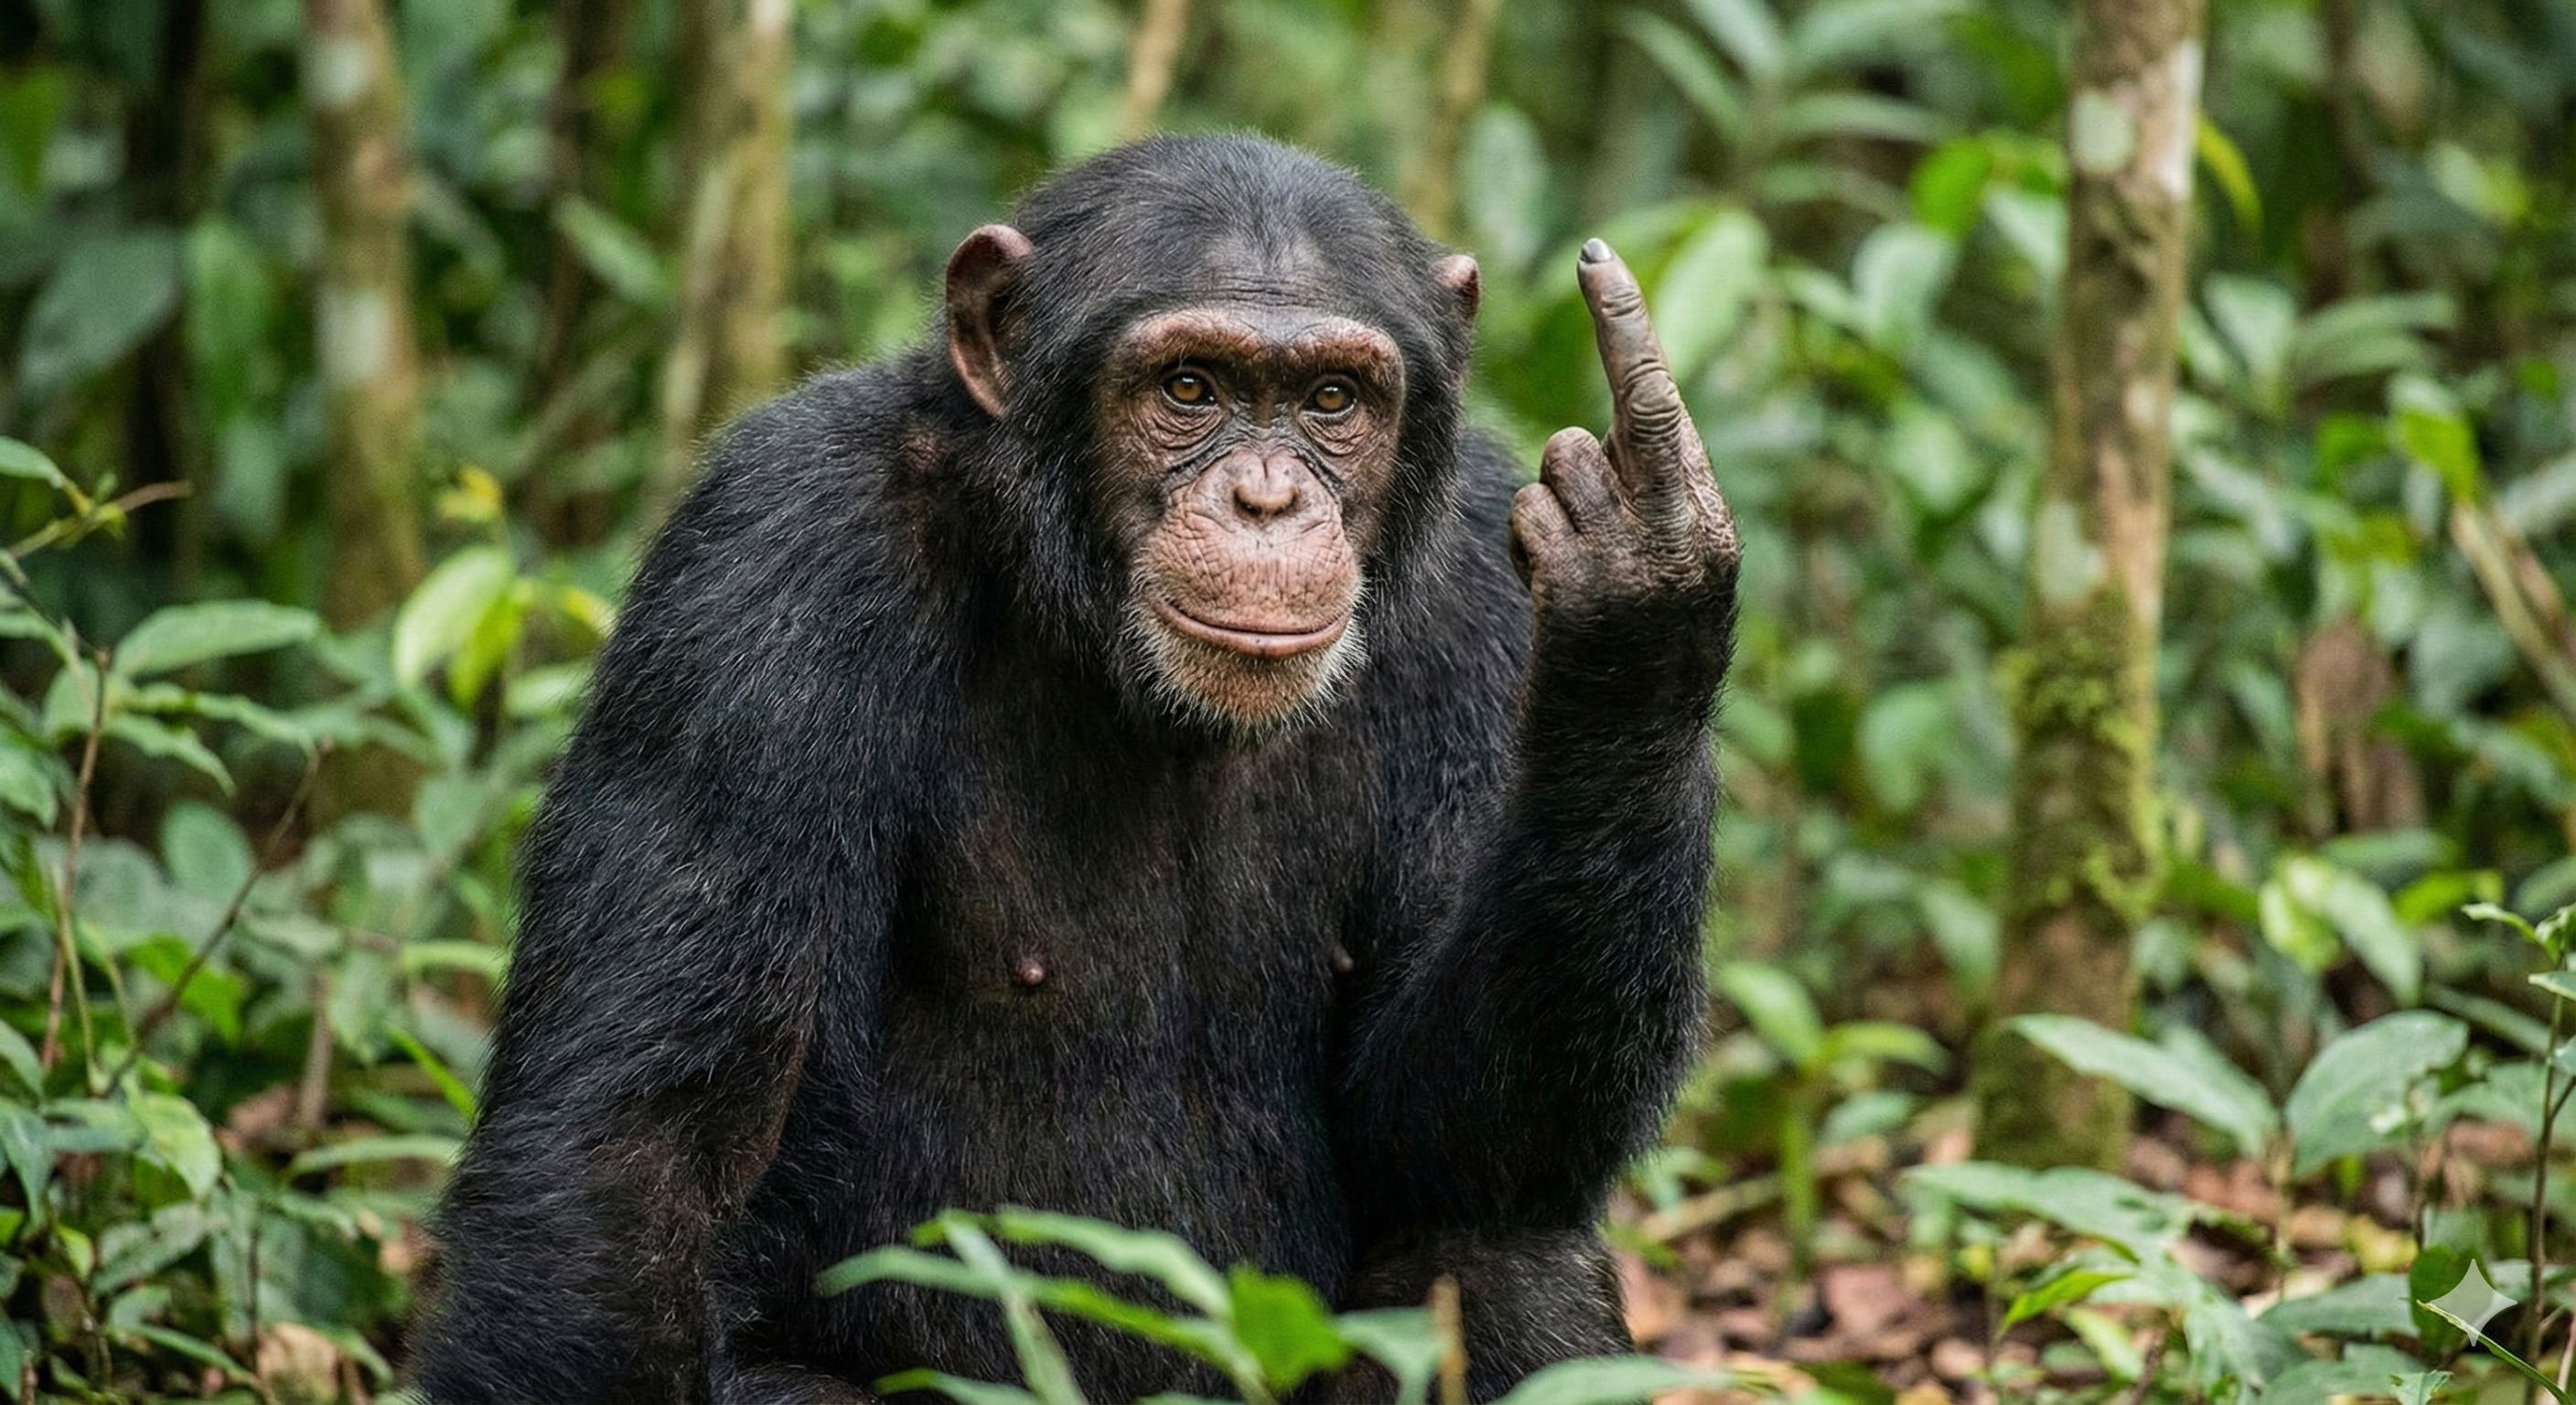
\includegraphics[scale = 0.1]{Assets/Image.png}
    \caption{Opice}
    \label{img:opice}
\end{figure}

V tomhle textu je potřeba něco\footnote{nebo taky ne} vysvětlit...

A tady níže lze spatřit \autoref{t:tabulka}.

\begin{table}[h!]
    \centering
    \caption{Pozdrav s indexováním od 0}
    \label{t:tabulka}
    \begin{tabular}{|l|l|}
        \hline
        \B{Sloupec 0} & \B{Sloupec 1} \\ \hline
        Ahoj & světe \\ \hline
        zdravím & z \\ \hline
        této & tabulky \\ \hline
    \end{tabular}
\end{table}

A tady někde v tomto textu lze napsat pomocí \TeX u jakýsi blok
kódu pomocí \cinline{\textbackslash cinline}.

Pokud si ovšem pečlivě prohlédneme ukázku \autoref{c:hovno}, zjistíme, že to je hovno. 

\cinput{Snippets/is3.py}{python}{c:hovno}{Hovno}

Dále tady také lze nají rovnice, jedním příkladem může být \autoref{e:wut}.

\eq{e:wut}{2 + 2 = 5}

\newpage